\documentclass[12pt,letterpaper]{article}
\usepackage[margin=.63in,headheight=15pt,headsep=19pt,footskip=25pt]{geometry}
\usepackage{tikz,fancyhdr,array}
\usetikzlibrary{arrows.meta}
\renewcommand{\familydefault}{\sfdefault}
\pagestyle{fancy}\fancyhf{}\renewcommand{\headrulewidth}{.4pt}
\fancyhead[L]{\small Week 20 / Averaging encore / Grades 2--5}
\fancyfoot[L]{\small Bellingham Math Circle / Week 20 / W20-BON-v1}\fancyfoot[R]{\small\thepage}
\setlength{\parindent}{0pt}\setlength{\parskip}{9pt}
\newcommand{\problem}[2]{\textbf{Problem #1:} #2\par}
\newcommand{\lines}[1]{\foreach \i in {1,...,#1}{\par\vspace{10pt}\hrulefill}\par}
\tikzset{circleplace/.style={draw,circle,minimum size=30mm,inner sep=0pt,fill=white},squareplace/.style={draw,rectangle,minimum size=30mm,inner sep=0pt,fill=gray!10}}
\newcommand{\pathmat}[4]{\begin{tikzpicture}[x=1cm,y=1cm]\draw (0,0)--(4,0)--(8,0)--(12,0);\node[squareplace] at (0,0){#1};\node[circleplace] at (4,0){#2};\node[circleplace] at (8,0){#3};\node[squareplace] at (12,0){#4};\end{tikzpicture}}
\newcommand{\cyclemat}[4]{\begin{tikzpicture}[x=1cm,y=1cm]\draw (0,0)--(3.5,0)--(3.5,3.5)--(0,3.5)--cycle;\node[circleplace] at (0,3.5){#1};\node[circleplace] at (3.5,3.5){#2};\node[circleplace] at (3.5,0){#3};\node[circleplace] at (0,0){#4};\end{tikzpicture}}
\begin{document}
A wandering token starts at a circle. At each move, choose fairly among all joined neighbors. Stop when it first reaches a square and record that square's score. A square with score 0 is still a possible choice.

\problem{1}{Run at least twelve walks starting at A, then twelve starting at B. What average score would you expect after many walks from each start? Use the same rule at C on the second board. Find exact expected scores for all three starts.}
\begin{center}\pathmat{0}{A}{B}{6}\end{center}
\begin{center}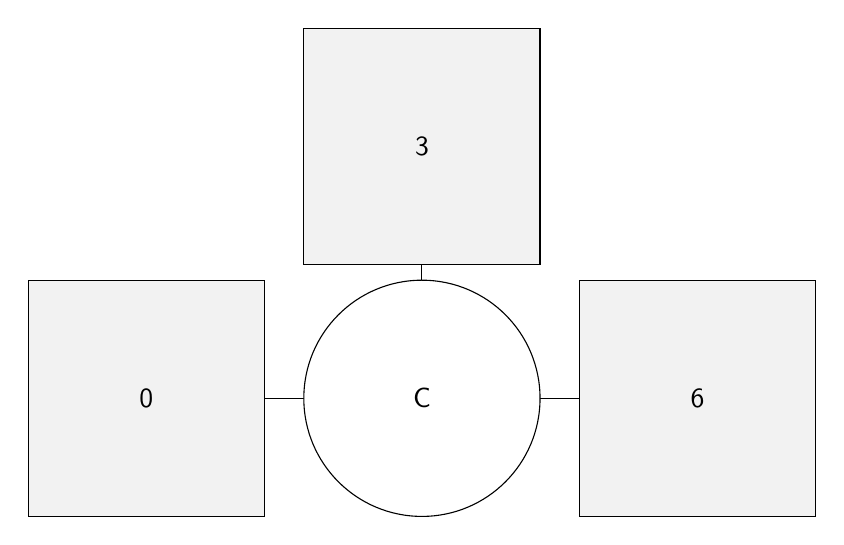
\begin{tikzpicture}[x=1cm,y=1cm]
\draw (0,0)--(-3.5,0) (0,0)--(3.5,0) (0,0)--(0,3.2);
\node[circleplace] at (0,0){C};\node[squareplace] at (-3.5,0){0};\node[squareplace] at (3.5,0){6};\node[squareplace] at (0,3.2){3};
\end{tikzpicture}\end{center}
\begin{center}\renewcommand{\arraystretch}{1.7}\begin{tabular}{c|p{4.9in}}
start&scores at the end of the walks\\\hline A&\\\hline B&\\\hline C&\\\hline
\end{tabular}\end{center}
\lines{2}
\newpage
At a tick, every circle takes the average of its neighbors' BEFORE values. Put all new values on a separate AFTER board. Then that whole board becomes the next BEFORE board. No value is fixed.

\begin{center}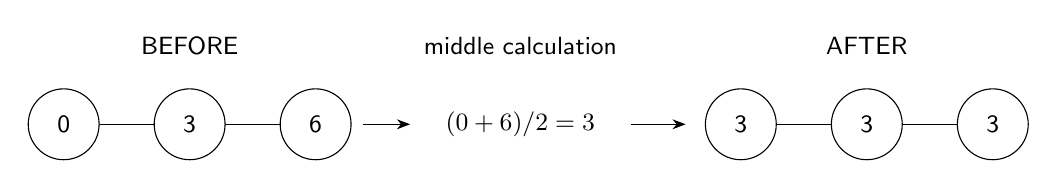
\begin{tikzpicture}[x=1cm,y=1cm]
\node at (1.6,1){\small BEFORE};\node at (5.8,1){\small middle calculation};\node at (10.2,1){\small AFTER};
\draw (0,0)--(3.2,0) (8.6,0)--(11.8,0);
\foreach \x/\v in {0/0,1.6/3,3.2/6,8.6/3,10.2/3,11.8/3}{\node[draw,circle,fill=white,minimum size=9mm] at (\x,0){\small\v};}
\node at (5.8,0){\small $(0+6)/2=3$};
\draw[-{Stealth}] (3.8,0)--(4.4,0);\draw[-{Stealth}] (7.2,0)--(7.9,0);
\end{tikzpicture}\end{center}

\problem{2}{Start with these four values. Keep updating the whole board until a state returns. Find a different starting state that also returns after exactly two ticks.}
\begin{center}\begin{minipage}{.48\textwidth}\centering\small BEFORE\par\cyclemat{0}{6}{0}{6}\end{minipage}\hfill\begin{minipage}{.48\textwidth}\centering\small AFTER\par\cyclemat{}{}{}{}\end{minipage}\end{center}
\begin{center}\renewcommand{\arraystretch}{1.6}\begin{tabular}{c|c|c|c|c}
tick&top left&top right&bottom right&bottom left\\\hline
0&0&6&0&6\\\hline 1&&&&\\\hline 2&&&&\\\hline 3&&&&\\\hline 4&&&&\\\hline
\end{tabular}\end{center}
\lines{2}
\newpage
Change the tick rule: average each circle's own BEFORE value together with all its neighbors' BEFORE values. Put all replacements on the AFTER board together.

\problem{3}{Start with two joined circles, 0 and 6. Compare repeated ticks using the rule from Problem 2 and the new rule above. Does either process settle to one unchanged board?}
\begin{center}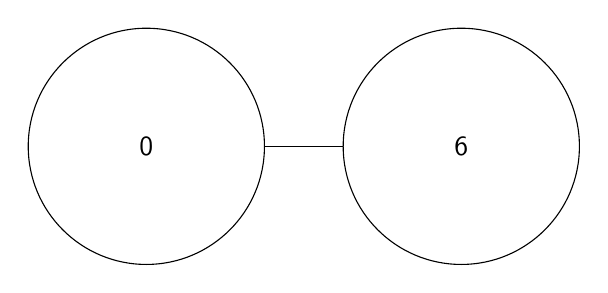
\begin{tikzpicture}[x=1cm,y=1cm]\draw (0,0)--(4,0);\node[circleplace] at (0,0){0};\node[circleplace] at (4,0){6};\end{tikzpicture}\end{center}
\lines{3}
\vspace{15pt}
\problem{4}{Use the new rule on the four-circle board starting at 0, 6, 0, 6. Find the next three whole boards. What value do you think each circle approaches? Can it reach that value exactly after a finite number of ticks?}
\begin{center}\renewcommand{\arraystretch}{1.8}\begin{tabular}{c|c|c|c|c}
tick&top left&top right&bottom right&bottom left\\\hline
0&0&6&0&6\\\hline 1&&&&\\\hline 2&&&&\\\hline 3&&&&\\\hline
\end{tabular}\end{center}
\lines{5}
\newpage
For a roughness score, find the gap between the two values on each edge. Make a square whose side is that gap. Add all the square areas, counting each edge once. Squares on the graph keep their values.

\begin{center}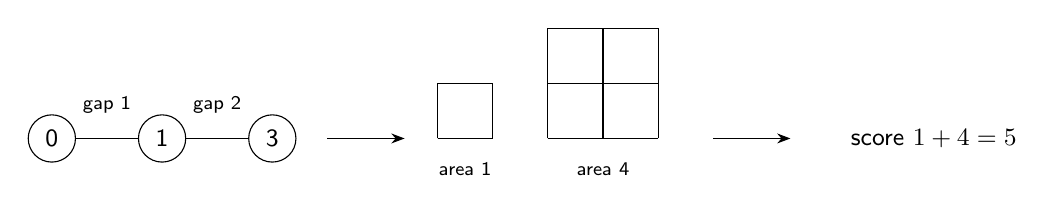
\begin{tikzpicture}[x=7mm,y=7mm]
\draw (0,0)--(2,0)--(4,0);\foreach \x/\v in {0/0,2/1,4/3}{\node[draw,circle,fill=white,minimum size=6mm] at (\x,0){\small\v};}
\node[font=\scriptsize] at (1,.6){gap 1};\node[font=\scriptsize] at (3,.6){gap 2};
\draw[-{Stealth}] (5,0)--(6.4,0);
\draw[step=1] (7,0) grid (8,1);\draw[step=1] (9,0) grid (11,2);
\node[font=\scriptsize] at (7.5,-.55){area 1};\node[font=\scriptsize] at (10,-.55){area 4};
\draw[-{Stealth}] (12,0)--(13.4,0);\node[font=\small] at (16,0){score $1+4=5$};
\end{tikzpicture}\end{center}

\problem{5}{Put a whole number from 0 to 6 at the circle. Find the smallest possible roughness score. Explain why no other choice gives a smaller score.}
\begin{center}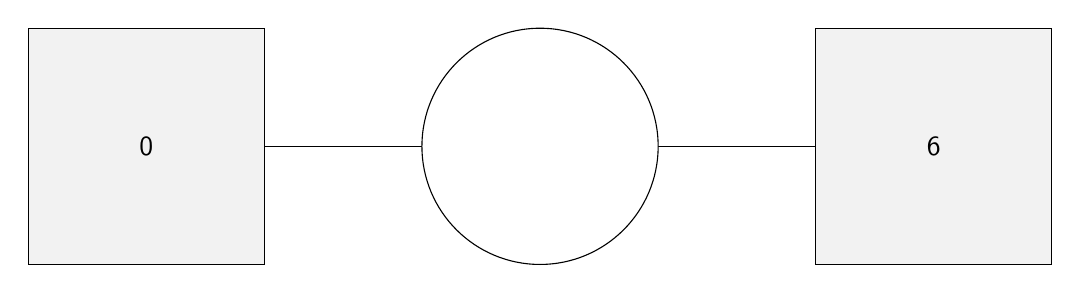
\begin{tikzpicture}[x=1cm,y=1cm]\draw (0,0)--(5,0)--(10,0);\node[squareplace] at (0,0){0};\node[circleplace] at (5,0){};\node[squareplace] at (10,0){6};\end{tikzpicture}\end{center}
\begin{center}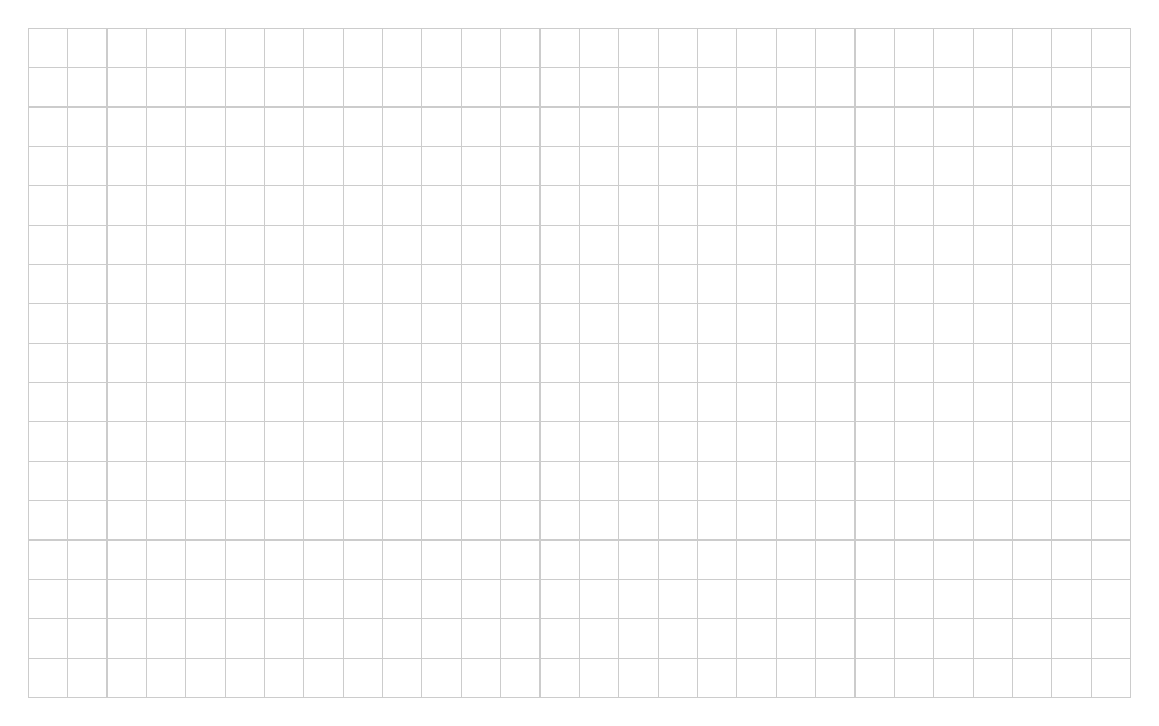
\begin{tikzpicture}[x=5mm,y=5mm]\draw[step=1,gray!40] (0,0) grid (28,17);\end{tikzpicture}\end{center}
\lines{2}
\newpage
\problem{6}{Choose whole-number values from 0 to 6 for the two circles. Make the roughness score as small as possible. Explain why your best score cannot be beaten.}
\begin{center}\pathmat{0}{}{}{6}\end{center}
\begin{center}\renewcommand{\arraystretch}{1.8}\begin{tabular}{p{1.1in}|p{1.1in}|p{2.2in}}
left circle&right circle&roughness score\\\hline
&&\\\hline &&\\\hline &&\\\hline &&\\\hline &&\\\hline
\end{tabular}\end{center}
\begin{center}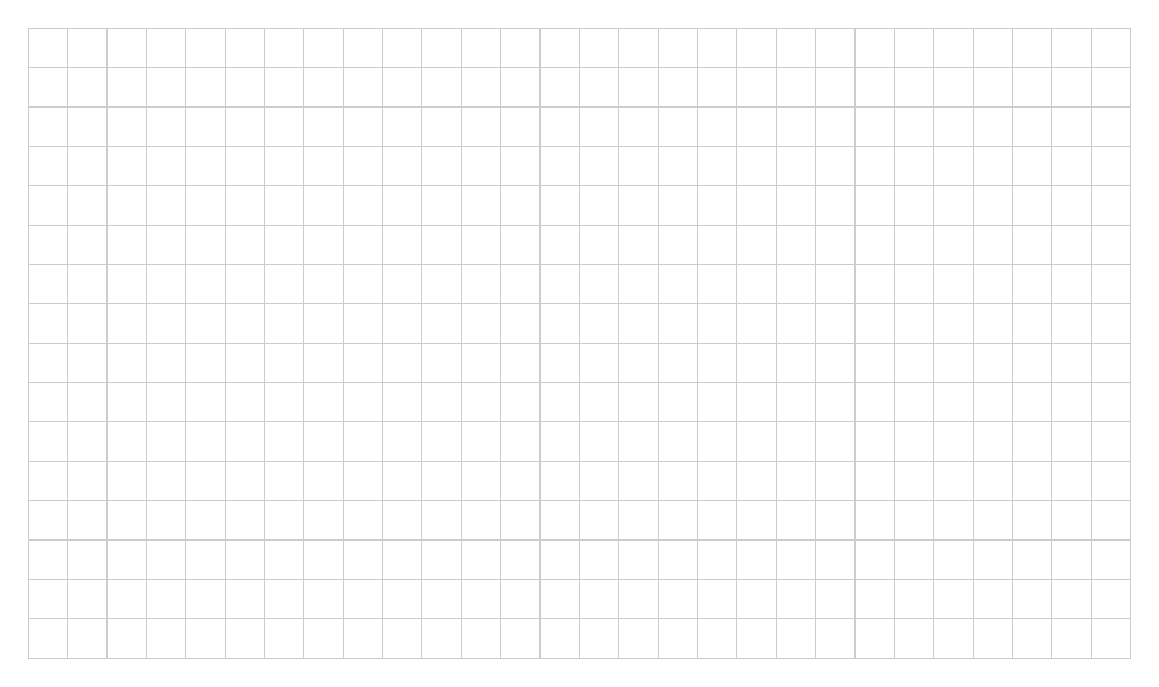
\begin{tikzpicture}[x=5mm,y=5mm]\draw[step=1,gray!40] (0,0) grid (28,16);\end{tikzpicture}\end{center}
\lines{2}
\end{document}
